\chapter{Диалоговая платформа DREAM}\label{ch:dream} 

Необходимость использования многозадачных нейросетевых моделей для обработки естественного языка обуславливает необходимость экономии вычислительных ресурсов при обрабоаатке естественного языка. Одной из ключевых областей, в которой широко применяются новейшие модели для обработки естественного языка, являются диалоговые системы.  Использование нейросетевых моделей, включая многозадачные, в диалоговых системах изучалось автором данном диссертационной работы на примере диалоговой системы DREAM, дважды принимавшей участие в конкурсе Alexa Prize Challenge, в качестве единственного российского решения за всю историю данного соревнования. Диалоговая система \texttt{DREAM} является полноценной диалоговой платформой, так как её исходный код после конкурсов был выложен в открытый доступ. Это позволяет использовать все технические решения, примененные при работе над данной платформой, сторонними разработчиками.

Автор диссертационной работы принимал активное участие в работе над диалоговой платформой DREAM. Так, автор оба раза был членом команды \texttt{DREAM} в конкурсе "Alexa Socialbot Grand Challenge", что описано также в работах \cite{dream1,dream1_trudy,dream2}. В данной главе описано устройство диалоговой платформы \texttt{DREAM} и её эволюция в течение двух конкурсов, при этом акцент по возможности сделан на ее компоненты, являющиеся личным вкладом автора. При этом личный вклад автора не исчерпывается работой только над упомянутыми в статье компонентами - он включал в себя также анализ работы других навыков диалоговой платформы и помощь в их отладке.

\textbf{Задачи} диссертационной работы, описываемые в данной главе:
\begin{enumerate}
  \item \textbf{Создать и выложить в открытый доступ диалоговую платформу DREAM, на которой в дальнейшем могло бы изучаться прикладное применение многозадачных нейросетевых моделей. Проверить качество этой диалоговой платформы международным конкурсом "Alexa Prize Socialbot Grand Challenge". }
  \item \textbf{Проверить применимость технологий, использованных в диалоговой платформе DREAM, в иных прикладных задачах.}
\end{enumerate}

\section{Конкурс “Alexa Prize Socialbot Grand Challenge”}

Компания Amazon проводит конкурс “Alexa Prize Socialbot Grand Challenge” с 2017 года. “Alexa Prize Socialbot Grand Challenge” - это конкурс диалоговых систем широкого профиля, разрабатываемых университетскими командами из разных стран. Данные системы могут общаться с пользователями голосовых колонок “Alexa” от Amazon на различные популярные темы. Режим разговора с диалоговой системой во время конкурса включается командой “Alexa, let’s chat”.

После окончания разговора пользователю предлагается оценить качество диалога по шкале от 1 до 5 ( 1 - наименьшая оценка, 5 - наибольшая). 

Финальная цель данного конкурса - добиться следующих показателей: среднее качество диалога больше 4, среднее время разговора больше 20 минут. Данные показатели на сегодняшний момент находятся за пределами возможностей всех университетских команд. По причине данного фактора, конкурс является поэтапным. Каждый год компания Amazon организует “Alexa Prize Challenge”, в котором из большого числа заявок (несколько сотен в год) отбирается до 10 университетских команд для участия в конкурсе.

Данный конкурс имеет продолжительность более полугода и состоит из следующих этапов:
\begin{itemize}
\item[*] Подготовительный период. Команды работают над своими диалоговыми системами и тестируют их внутри своих команд.
\item[*] Период бета-тестирования на пользователях-сотрудниках “Amazon”. 
\item[*] Период начальной обратной связи (англ: Initial Feedback Period). В этот период системы-участники впервые становятся доступными обычным пользователям колонок, которые могут общаться с этими системами и ставить им ту или иную оценку. Рейтинги в этот период еще не влияют на отбор команд для прохода в следующий этап.
\item[*] Период четвертьфинала(англ: Quaterfinals). По рейтингам за последнюю неделю четвертьфиналов отбираются команды для прохода в полуфиналы.
\item[*] Период полуфинала(англ: Semifinals). По среднему рейтингу за все время полуфиналов отбираются команды для прохода в финалы.
\item[*] Период финала(англ: Finals). Во время финалов специально обученное жюри проводит слепое тестирование диалоговых систем. По результатам данного тестирования жюри выбирает итогового победителя. При этом изменения кода в периоде финалов уже запрещены.
\end{itemize}

Команда Московского физико-технического института “DREAM” была отобрана для участия в конкурсах “Alexa Prize Challenge 3” \cite{na_website_ndh} и “Alexa Prize Challenge 4” \cite{na_website_ndi}. В каждом из этих конкурсов автор данной диссертационной работы принимал активное участие в этой команде. Диалоговая система \texttt{DREAM} подробнее описана в \cite{dream1}\cite{dream1_trudy}\cite{dream2}.

\begin{figure}[ht]
  \centerfloat{
    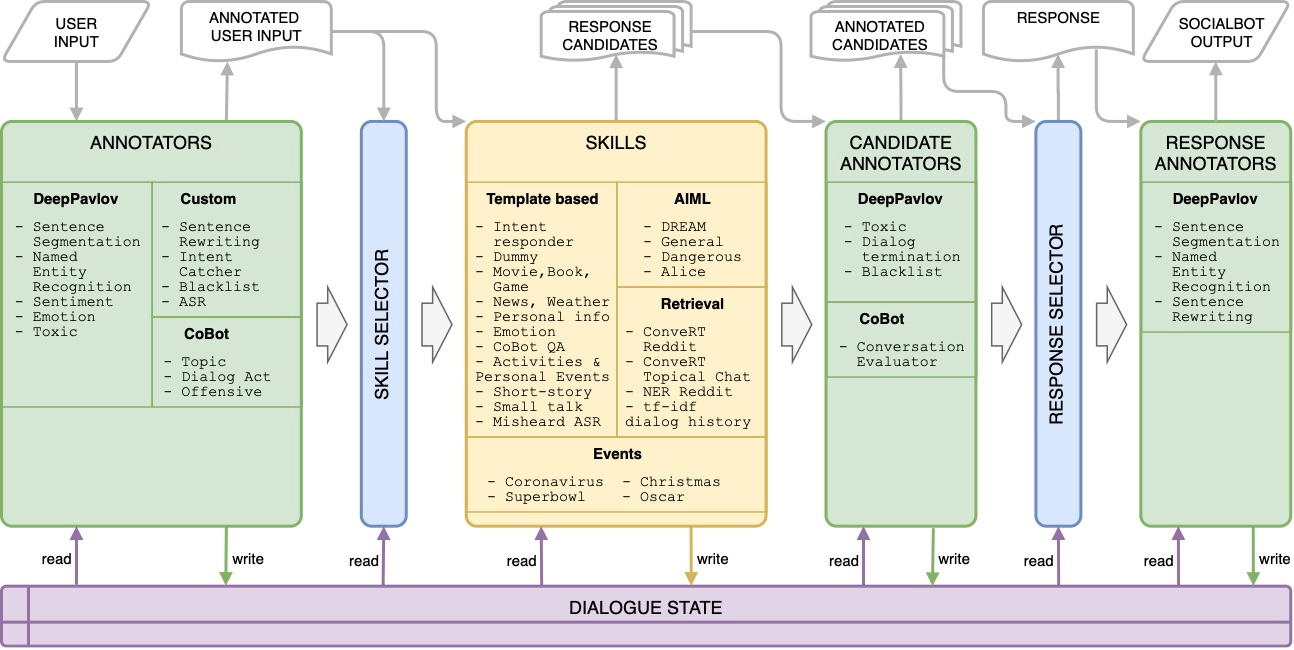
\includegraphics[width=\textwidth]{images/Alexa1_.png}
  }
  \caption{Архитектура диалоговой системы \texttt{DREAM} в конкурсе “Alexa Prize Challenge 3”}\label{fig:Alexa1}
\end{figure}


Диалоговая система \texttt{DREAM} для участия в конкурсе “Alexa Prize Challenge 3” разрабатывалась с нуля, на основе фреймворка “DeepPavlov Agent” -  разработки сотрудников лаборатории нейронных систем и глубокого обучения МФТИ. Разработка \texttt{DREAM} велась с 2019 года.

В связи с тем, что “DeepPavlov Agent” на тот момент находился на раннем этапе своего развития, код “DeepPavlov Agent” был скопирован непосредственно в репозиторий диалоговой системы и редактировался непосредственно в этом репозитории.  

Задача развертывания диалоговой системы на большое число пользователей решалась с использованием Docker Compose. \cite{na_website_ndk}

На Рисунке \ref{fig:Alexa1} представлена верхнеуровневая архитектура диалоговой системы \texttt{DREAM} на момент завершения ее участия в конкурсе "Alexa Prize Challenge 3". Реплика, поступающая модели \texttt{DREAM} на вход, вместе с Dialog State(в котором хранится информация о диалоге вместе со всеми аннотациями) проходит через аннотаторы(Annotators). На основе аннотаций, полученных от аннотаторов, модуль Skill Selector, пользуясь оригинальным алгоритмом, выбирает навыки для генерации кандидатов на возможный ответ бота. Каждый навык генерирует возможный ответ с определенной степенью уверенности. Данные ответы фильтруются при помощи аннотаторов кандидатов на ответ, этим ответам присваиваются очки от модуля Cobot. На основе аннотаций, очков и фильтрации оригинальный разработанный модуль Response Selector выбирает финальный ответ-кандидат. Данный ответ проходит через постаннотаторы и в таком виде уже доводится до пользователя.

Диалоговая система принимает реплики пользователя на вход в виде текстовой транскрипции. При этом модуль тестовой транскрипции предоставляется компанией Amazon “из коробки”. Заметим, что ошибки этого модуля сами являлись причиной определенного процента ошибок диалоговой системы DREAM(около 10 процентов).

На вход модели, после каждой реплики пользователя, поступает список слов, которые распознала модель. Каждому слову соответствует степень уверенности распознавания речи. Например, после фразы пользователя "alexa how old are you" модель получает на вход от модуля текстовой транскрипции список следующего вида: [(“alexa”: 0.95), “how”:0.96, (“old”:0.8), (“you”: 0.9)]. Заметим, что подобные списки не разделены по предложениям и не имеют пунктуацию. Поэтому, чтобы реплики обрабатывались лучше, диалоговая система использует аннотатор Sentence Segmentation для восстановления пунктуации и разделения реплик на предложения. Кроме этого диалоговая система использует также модель Sentence Rewriting, заменяющую местоимения на сущности, которые были упомянуты ранее в диалоге.


\subsection{Первый этап разработки: навыки и аннотаторы}

На первом этапе разработки ключевыми интегрированными в бота \texttt{DREAM} навыками и аннотаторами, помимо упомянутых выше, являлись:

Удаленные сервисы, предоставленные командой “Amazon” -  классификатор тем Cobot Topics, классификатор диалоговых актов и тем Cobot DialogAct, вопросно-ответная система Cobot QA

Имеющиеся в открытом доступе навыки для диалога на общие темы, построенные на правилах - Alice, AIML Chit-Chat(встроенный под названием program-y). В дальнейшем данные навыки многократно совершенствовались - как в связи с паттернами ответов пользователей, наблюдавшихся в реальных диалогах с системой DREAM, так и в связи со специфичными требованиями правил \cite{na_website_ndg}. Помимо этого, был добавлен навык Intent Responder для ответа на конкретные интенты и навыки-”затычки” Dummy Skill и Dummy Skill Dialog.

\subsection{Аннотаторы}

На следующих этапах разработки добавлялись иные аннотаторы реплик пользователя, часть из которых ( см. Рисунок 10) также использовалась как постаннотаторы для аннотации реплик диалоговой системы. Такие аннотаторы включают в себя:
\begin{itemize}
\item[*] Blacklisted Words Detector - используется для обнаружения нецензурных или просто оскорбительных слов или выражений. Данный аннотатор основан на регулярных выражениях и использует заданный вручную список слов.

\item[*] Intent Catcher - используется для обнаружения одного из 22 интентов. Данный аннотатор работает как на наборе регулярных выражений, обновлявшемся вручную в течение конкурса, так и на модели Universal Sentence Encoder \cite{cer_2018}.

\item[*] Toxic Classification - нейросетевой многометочный классификатор, определяющий, относится ли реплика к любому из следующих классов - ненависть(identity\_hate), оскорбление(insult), обсценная лексика(obscene), очень токсичный(very\_toxic), секс(sexual\_explicit), угроза(threat), токсичный(toxic). Данный аннотатор основывается на модели "разговорный BERT"\cite{dp_conv_bert}, которая является частью библиотеки DeepPavlov и которая была дообучена на данных с Kaggle-соревнования "Jigsaw Unintended Bias in Toxicity Classification" \cite{toxic_kaggle}.

\item[*] Sentiment Classification - нейросетевой классификатор тональности, основанный на модели “разговорный BERT” \cite{na_website_ndn}, обученной на наборе данных Stanford Sentiment Treebank \cite{sst}. Классификатор распознает три класса - положительный, отрицательный, нейтральный.

\item[*] Dialog Termination - нейросетевой классификатор - предсказатель завершения диалога. Ближе к концу конкурса, когда у команды \texttt{DREAM} накопилась достаточно большая база диалогов(сотни тысяч), на основе вышеупомянутой модели “разговорный BERT” была обучена модель-постаннотатор, которая для каждой реплики бота определяла вероятность завершения пользователем диалога после этой реплики. На основании очков от этой модели Response Selector фильтровал реплики-кандидаты. Данная модель является личным вкладом автора диссертационной работы.

\item[*] Emotion Classification -  нейросетевой классификатор эмоций, основанный на модели “BERT-Base-uncased”, обученный на наборе данных с Kaggle страницы Eray Yildiz \cite{na_website_ndp_emo}. Эти данные содержали 6 классов - ярость, грусть, любовь, радость,удивление, любовь. Для корректной работы классификатора необходимо, чтобы в данных присутствовали также примеры, принадлежащие нейтральному классу. Для этого были добавлены примеры из набора данных ScenarioSA \cite{scenariosa}, которым был присвоен нейтральный класс. Итоговый набор данных сохранен по адресу \cite{na_website_ndo_emo}.
\end{itemize}
Модель \textbf{Emotion Classification} является личным вкладом автора, в связи с чем она описывается более подробно, чем остальные. После первой эпохи при обучении с оптимизатором Adam и скоростью обучения 5*10-5 данной моделью была достигнута точность 94.2\% на валидационном наборе данных. Классификатор обучался как многометочный, но для метрик предсказанным считался самый вероятный класс. Матрица ошибок данного классификатора представлена ниже.


\begin{table}[htbp]
\centering
\caption {Матрица ошибок классификатора эмоций из Alexa Prize Challenge 3}
\label{tab:dream1}% label всегда желательно идти после caption
\resizebox{\textwidth}{!}{%
\begin{tabular}{|c||c|c|c|c|c|c|c|}
\hline
\begin{tabular}[c]{@{}l@{}}Предсказанный класс\\----------\\Настоящий класс\end{tabular}  & Ярость & Страх & Удовольствие & Любовь & Грусть & Удивление & Нейтральный\\
\hline
\hline
Ярость & 5933 & 49 & 38 & 2 & 22 & 291 & 1 \\
\hline
Страх & 263 & 4624 & 18 & 0 & 12 & 1 & 419 \\
\hline
Удовольствие & 17 & 5 & 14697 & 1138 & 4 & 27 & 112 \\
\hline
Любовь & 1 & 1 & 14 & 3867 & 0 & 4 & 1 \\
\hline
Грусть & 6 & 3 & 2 & 1 & 3109 & 0 & 0 \\
\hline
Удивление & 48 & 229 & 36 & 7 & 9 & 13725 & 16 \\
\hline
Нейтральный & 1 & 2 & 44 & 0 & 0 & 2 & 1609 \\
\hline
\end{tabular}
}
\end{table}



Результат данного классификатора в данном конкурсе использовался навыками обсуждения эмоций и обсуждения коронавируса, которые будут подробнее описаны в разделе \ref{dream:1:closed}.

Последние 4 описанных модели основаны на подходе, описанном в главе данной диссертации “Предварительно обученные языковые модели” с дообучением данных языковых моделей на конкретную задачу. 

\subsection{Навыки открытого домена}

В течение конкурса командой \texttt{DREAM} активно создавались навыки открытого домена для того, чтобы как можно большее число тем было покрыто хотя бы на минимальном уровне. Были созданы следующие навыки открытого домена:

TF-IDF Retrieval использует диалоги за прошлый месяц, получившие хорошую оценку (5) и плохую (1-2). Получая на вход пользовательскую фразу, он строит TF-IDF векторное представление данной фразы и выбирает фразу бота из получивших хорошую оценку диалогов, максимально близкую по косинусному расстоянию к данной пользовательской фразе и не принадлежащую при этом к множеству диалогов, получивших плохую оценку. Уверенность данного навыка соответствует косинусному расстоянию между векторными представлениями фразы пользователя и бота, но не превышает при этом некоторе постоянное значение. Векторизатор для получения представлений был обучен на конкатенации наборов данных TopicalChat\cite{topicalchat}, PersonaChat \cite{personachat} и Wizard of Wikipedia \cite{wow}. Разработка данного навыка относится к личному вкладу автора.  Это единственный навык, который интегрировал в себя новые диалоговые данные из конкурса в автоматическом режиме.

В дальнейшем было также обучено подмножество аналогичных навыков, покрывающих разные темы из набора данных TopicalChat  - книги, развлечения, мода, фильмы, музыка, политика, технологии, спорт и животные - каждый на основе соответствующего набора данных из TopicalChat.

Генеративный навык является другой разработкой автора. В данном навыке использовалась модель типа GPT\cite{radford_2018_gpt} с добавлением “персоны” для улучшения качества генерации модели. Данная модель дообучалась в различных экспериментах на PersonaChat, на TopicalChat, на Wizards of Wikipedia или на сочетании всех этих трех наборов данных . В качестве персоны(сообщения, исходя из которого генерировалась дальнейшая реплика) в данных экспериментах использовались в качестве условия для генерации, соответственно, персона для примеров из набора данных PersonaChat, одно из предложений, на которое была отсылка в Wizards of Wikipedia(далее - WOW) для примеров из Wizards of Wikipedia и один из наиболее релевантных фактов, связанных с этой фразой(по TF-IDF) для примеров из TopicalChat. Максимальная длина предложения со всей диалоговой историей и персоной равнялась 512 токенов.  Данная модель продолжает проводившуюся ранее автором работу над диалоговой моделью “с персоной” \cite{Болотин_Карпов_Рашков_Шкурак_2019}.

Несмотря на хорошие результаты по метрике perplexity(см. таблицу ниже ~\ref{tab:dream2}), навык не был включен в систему \texttt{DREAM} из-за своей недостаточной логической консистентности.


\begin{table}[htbp]
\centering
\caption {Точность (перплексия) для генеративного навыка}
\label{tab:dream2}% label всегда желательно идти после caption
\resizebox{\textwidth}{!}{%
\begin{tabular}{|c||c|c|c|c|}
\hline
Модель & \begin{tabular}[c]{@{}l@{}}Метрики\\(PersonaChat)\end{tabular} & \begin{tabular}[c]{@{}l@{}}Метрики\\(TopicalChat)\end{tabular} & \begin{tabular}[c]{@{}l@{}}Метрики\\(WOW)\end{tabular} &\begin{tabular}[c]{@{}l@{}}Метрики\\(3 набора данных)\end{tabular}\\
\hline \hline
GPT (PersonaChat) & 90(12.3) & - & - & - \\
\hline
GPT (Topical-Chat) & - & 96(9.7) & - & - \\
\hline
GPT (WOW) & - & - & 86.7(27.2) & - \\
\hline
GPT (3 набора данных) & 86(14.2) & 92(11.6) & 83(31.5) & 92(16.3) \\
\hline
\end{tabular}
}
\end{table}



ConveRT Reddit - нейросетевой ранжирующий навык, обученный на наборе комментариев с сайта REDDIT \cite{na_website_ndu} (отфильтрованном аннотаторами Cobot Conversation Evaluator и Toxic Classifier до 80 тыс.примеров) и использующий нейросетевую модель CONVERT \cite{henderson_2019} для получения векторных представления реплики и контекста(конкатенации предыдущих реплик). Данная модель вместо модели BERT была выбрана в целях экономии вычислительных ресурсов и для повышения быстродействия.

\subsection{Навыки закрытого домена}\label{dream:1:closed}

Тем не менее, вышеупомянутых навыков все еще в большинстве случаев было недостаточно для того, чтобы вести долгий, логически завершенный диалог на популярные темы. В связи с этим также был создан ряд навыков закрытого домена, основанных на правилах, использовании нейросетевых аннотаций и при необходимости делающий внешние запросы. Такие навыки, как Movie Skill, Game Skill, News Skill, Weather Skill, Small Talk Skill, Personal Info Skill, News Skill, Christmas Skill, Valentine’s Day Skill, Superbowl Skill, Oscar Skill, подробно описаны в \cite{dream1} и \cite{dream1_trudy}. Ниже будут описаны три навыка закрытого домена, являющихся личным вкладом автора.

Emotion Skill возвращает шаблонные ответы на эмоции, обнаруженные аннотатором Emotion Classification. В частности, навык может подсказать совет,рассказать шутку или успокоить пользователя. Основная часть навыка была разработана автором самостоятельно.

В начале февраля 2020 года года, несмотря на общее падение рейтингов диалоговой системы(вероятно, связанное  с беспокойством пользователей по поводу новой коронавирусной инфекции), улучшение навыка Emotion Skill помогло повысить медианное время диалога с 58 до 73 секунд.

Book Skill, используя базу данных Amazon Evi \cite{na_website_nds}, находит названия книг и фамилии авторов. Используя данные именованные сущности, навык поддерживает разговор о данных книгах либо авторах. Помимо этого, навык также может рекомендовать книги, используя информацию из базы данных GoodReads \cite{na_website_ndt} и аннотации из модели Cobot. Одной из технических проблем при разработке данного навыка являлось то, что некоторые названия книг заставляли реагировать и Book Skill, и Emotion Skill. Проблема была решена при помощи изменения уверенности навыка Book Skill в таких ситуациях.

В работе \cite{dream1} показано, что использование Book skill и описанного выше TF-IDF Retrieval помогло повысить рейтинг диалоговой системы в декабре 2019 года с 3.01 до 3.19.  В конце января-начале февраля 2020 года добавление истории диалога в TF-IDF Retrieval помогло дополнительно повысить рейтинг диалоговой системы до 3.25. 

Coronavirus Skill был добавлен на завершающем этапе конкурса, когда в связи с эпидемией COVID-19 (дело происходило в марте-июне 2020 года) пользователи стали часто поднимать эту тему в разговорах с диалоговой системой DREAM. Навык использовал данные о случаях коронавируса и смертях от него, взятых из Центра системной научной инженерии Университета Джона Хопкинса \cite{na_website_ndr}. Навык использует факты, сравнения и научно обоснованные советы для того, чтобы успокоить пользователя с учетом его возраста. Навык использует аннотации от Emotion Classification.

 Прирост рейтинга диалоговой системы в начале марта 2020 года был, вероятно, связан с добавлением и улучшением навыка Coronavirus Skill.

\subsection{Response Selector и Skill Selector}

При большом числе сценарных навыков, у многих пользователей тем не менее в середине конкурса возникали трудности с тем, чтобы “попасть” в какой-то конкретный навык. В связи с этим диалог часто становился логически неконсистентным. Для решения данной проблемы был реализован метод “направляющих вопросов”, подразумевающих в качестве ответа мнение пользователя о заданной теме и/или выбор пользователем конкретной темы для обсуждения ( фильма, книги, игры). Данные вопросы могли добавляться как на уровне навыка, так и на уровне Response Selector. Как показано в \cite{dream1}, использование подобного метода помогло повысить рейтинг диалоговой системы.
Алгоритм выбора навыков Skill Selector основан на постоянном включении нетематических навыков, включении тематических навыков при определенных условиях на аннотации реплики пользователя и использовании специального режима при обработке реплик, классифицированных Toxic Classification как токсичные или просто принадлежащим к “острым” темам. Подробнее данный алгоритм описан в работе \cite{dilya_thesis}.
Алгоритм выбора ответа Response Selector в начале участия команды \texttt{DREAM} в конкурсе просто выбирал навык с максимальной уверенностью. В дальнейшем туда были интегрированы оценки от Cobot Conversation Evaluator, фильтрация с использованием постаннотаторов и набор иных эвристик. Подробнее данный алгоритм описан в той же работе \cite{dilya_thesis}.

\section{Архитектура диалоговой системы \texttt{DREAM} в “Alexa Prize Challenge 4”}


\begin{figure}[ht]
  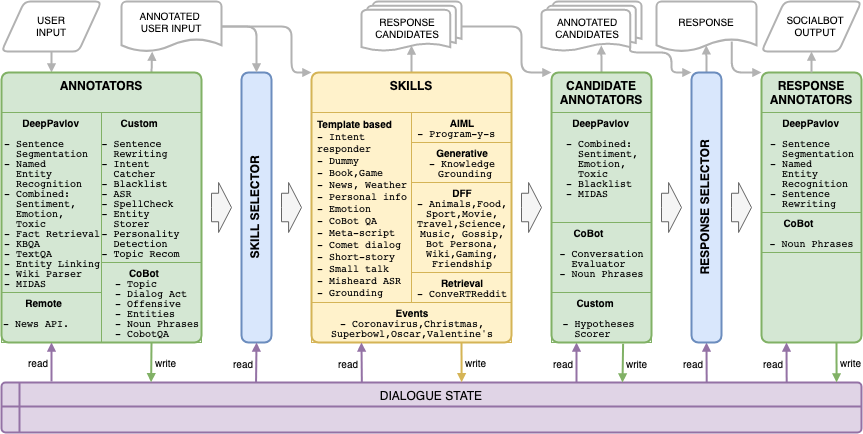
\includegraphics[width=\textwidth]{images/Alexa2_.png}
  \caption{Архитектура диалоговой системы \texttt{DREAM} в конкурсе “Alexa Prize Challenge 4”}\label{fig:Alexa2}
\end{figure}
Диалоговая система \texttt{DREAM} для участия в конкурсе следующего, 2021 года основывалась на доработанной системе прошлого года. Её схема представлена на рисунке \ref{fig:Alexa2}.


Задача развертывания диалоговой системы решалась с использованием Kubernetes. \cite{kubernetes}
Ключевые принципы работы диалоговой системы остались прежними, однако ее аннотаторы и навыки поменялись следующим образом.

\subsection{Изменения, связанные с аннотаторами}\label{dream:2:ann}

Одним из главных изменений, сделанных в диалоговой системе DREAM, являлась оптимизация вычислительных мощностей для экономии видеопамяти. Это было связано с высокими издержками на эксплуатацию данных мощностей - каждый месяц расходовалось “кредитов” вычислительных мощностей на сумму до 9 тысяч долларов США. Для данной оптимизации шесть моделей-классификаторов: Emotion Classifier, Sentiment Classifier, Toxic Classifier, Cobot Topic Classifier и Cobot DialogAct Classifier (последний классификатор считался за 2, т.к возвращал тему и интент) были объединены в один классификатор Combined Classifier. В условиях острого дефицита временных ресурсов, связанного с быстрой динамикой конкурса, был выбран способ реализации многозадачного обучения “Независимые метки” из статьи  \cite{pseudolabel}, описанный также в главе \ref{ch:pseudolabel}. Подробнее эксперименты, связанные с обучением данной модели, описаны ниже в главе \ref{ch:mtldream}. Данная модель использовалась как постаннотатор всё время конкурса, а как классификатор пользовательских фраз - при условии, что получение аннотаций от CoBot невозможно или задерживается(т.к модель CoBot имеет лимит на количество входящих запросов, такие ситуации возникали),  Данная модель является личным вкладом автора диссертационной работы.

Другим важным изменением является добавление модели для классификации диалоговых актов MIDAS Classifier, обученной на базе набора данных MIDAS \cite{midas}. На первом этапе, в феврале, была интегрирована предоставленная авторами модель, на втором, в апреле, она была заменена собственной моделью, обученной только на семантических классах из данного набора данных, так как в модели \texttt{DREAM} используется только этот набор классов.


Полный список используемых семантических классов:
\begin{itemize}
\item[*] открытый вопрос/мнение (open\_question\_opinion)
\item[*] открытый личный вопрос(open\_question\_personal)
\item[*] вопрос да/нет(yes\_no\_question)
\item[*] вопрос для пояснения(clarifying\_question)
\item[*] команда(command)
\item[*] неверная команда (dev\_command)
\item[*] признательность(appreciation)
\item[*] мнение(opinion)
\item[*] жалоба(complaint)
\item[*] комментарий(comment)
\item[*] утверждение(statement)
\item[*] другие ответы(other\_answers)
\item[*] положительный ответ(pos\_answer)
\item[*] отрицательный ответ(neg\_answer)
\item[*] открытый фактический вопрос(open\_question\_factual)
\end{itemize}
Обе модели были обучены на основе вышеупомянутой модели “разговорный BERT”.  Работа над данным аннотатором тоже является личным вкладом автора диссертационной работы. 

В конце февраля-начале марта 2021 года, как показано  в работе \cite{dream2}, интеграция Midas Classification и изменение модели диалога в сторону более частого показа Book Skill помогли поднять рейтинг диалоговой системы \texttt{DREAM} с ~3.11 до ~3.28.



Помимо этого, с середины конкурса использовался аннотатор Cobot Entities от Amazon как удаленный сервис. Данный аннотатор извлекал сущности и классифицировал их на несколько видов.
Также для рекомендации пользователю следующей темы (поддерживаемой имеющимся сценарным навыком) на основании текущего контекста был создан аннотатор Topic Recommendation, подробно описанный в \cite{dream2}.
Одним из ключевых изменений стала интеграция баз знаний - добавление компонентов Entity Linking, Wiki Parser и Fact Retrieval.Компонент Fact Retrieval получает для распознанных Cobot Entities сущностей факты из Википедии и WikiHow \cite{wikihow}.  Компонент Entity Linking соотносит каждую сущность, распознанную Cobot Entities, с идентификатором в системе WikiData \cite{vrandei_2014}. Компонент Wiki Parser извлекает из этих идентификаторов триплеты - наборы (субъект, соотношение, объект). Entity Linking и Wiki Parser широко использовались в навыках закрытого домена, таких, как Book Skill и Gossip Skill, что позволило существенно улучшить их качество работы.
Также из всех навыков, которые делали запрос к удаленным сервисам(пример -  Cobot QA, News API Skill), модули запросов были оформлены как отдельные аннотаторы, что позволяло делиться полученной информацией между навыками.
Для того, чтобы определять, задал ли пользователь фактоидный вопрос ( что в соответствии с алгоритмом, описанным в \cite{dream2}, определяет приоритетность включения части упомянутых выше навыков), был также добавлен аннотатор Factoid Classification. Этот аннотатор был основан на модели BERT, обученной на наборе данных YAHOO ССЫЛКА.
Помимо добавления новых навыков, инкрементальным улучшениям подвергались и старые навыки. В частности, автор работы большое время посвятил работе над Intent Catcher. 

\subsection{Изменения, связанные со сценарными навыками}
Одной из ключевых проблем, с которыми сталкивалась диалоговая система \texttt{DREAM} на момент проведения конкурса “Alexa Prize Challenge 3”, являлось недостаточное количество сценарных навыков. (У команды-победителя сценарные навыки покрывали больше популярных тем на разговор хотя бы в несколько шагов, чем у команды DREAM). Те сценарные навыки, которые были реализованы, не были унифицированы распространялись на другие темы, в связи с чем качество разговоров бота на многие темы были низкими, также возникали сложности с отладкой навыка человеком, который его не разрабатывал. Для решения этой проблемы Денисом Кузнецовым был разработан фреймворк для построения диалоговых систем Dialog Flow Framework(DFF) \cite{dff}, позволяющий удобно записывать сценарий для диалогового графа. На основе данного фреймворка было разработано большое количество сценарных тематических навыков - Animals Skill, Food Skill, Sport Skill, Science Skill, Music Skill, Gossip Skill, Gaming Skill, Bot Persona Skill, Travel Skill, а также переведен на использование DFF навык Movie Skill. Разработка подобных сценарных навыков позволила отключить использование соответствующих ранжирующих навыков, основанных на TF-IDF.

Личным вкладом автора диссертационной работы на данном этапе является существенное улучшение навыков Book Skill(на основе запросов к Wikidata), Emotion Skill и аннотатора Intent Catcher. 

Помимо Book Skill, Coronavirus Skill и Emotion Skill,автор диссертационной работы отвечал еще за 2 сценарных навыка.
Одним из этих навыков был Grounding Skill. Навык решал задачу установления взаимопонимания с пользователем. Используя информацию из истории диалога о том, какие сущности были упомянуты и какие были намерения у пользователя и у бота, навык генерирует шаблонную фразу-подтверждение. Этой фразой навык показывает, что бот понимает, о чем говорит пользователь. Например, если в аннотациях фразу есть сущность Fortnite и интент Opinion\_RequestIntent, навык выдает фразу “You wanted to hear my thoughts about Fortnite, am I correct?"

Другим навыком являлся Gossip Skill. В этом навыке отношение диалоговой к различным знаменитостям определялось случайно, и навык, используя WikiData и тональность реплики пользователя при его разговоре о той или иной знаменитости, обсуждал их. За работу над этим навыком автор диссертационной работы отвечал не все время(в отличие от первого навыка), но значительную часть времени.

\subsection{Изменения, связанные с навыками открытого домена}

Хотя сценарные навыки позволили вести логически связный разговор с пользователем значительное число диалогов и улучшить тем самым рейтинг этих диалогов, они все еще не могли покрыть все популярные темы и их подтемы. Для решения данной задачи были разработаны следующие навыки открытого домена, помимо упомянутых выше:
\begin{itemize}
\item[*] Knowledge Grounding Skill - нейросетевая генеративная модель ParlAI Blender 90M \cite{roller_other_2020}, дообученная на наборе диалогов Topical Chat Enriched \cite{hedayatnia_2020}.
\item[*] Wiki Skill - универсальный сценарный навык открытого домена. Он может обсуждать найденные в репликах пользователя сущности с использованием соответствующей страницы Википедии, что позволяет вести логически консистентный диалог по большому количеству популярных объектов, которые находятся за пределами внимания сценарных навыков.
\end{itemize}
\subsection{Изменения Response Selector и Skill Selector}

Ключевые изменения в Response Selector и Skill Selector включали в себя более плавные переходы между парами тем; использование специфичных переходных фраз, относящихся к 2 темам одновременно, либо обычных связующих фраз как во время конкурса “Alexa Prize Challenge 3”, но вместе со связующими фактами. 
Помимо этого, в связи с ростом количества и разнообразия сценарных навыков одной только уверенности перестало хватать для определения очередности их включения. В связи с этим сценарные навыки была добавлена приоритизация с возможными флагами продолжения “can continue”, “can not continue” и “must continue”.
Подробнее обо всех изменениях в алгоритмах Response Selector и Skill Selector можно прочитать в работе \cite{baymurzina_2021}.

\section{Проверка применимости технических решений, используемых в диалоговой платформе DREAM, в сторонних задачах}

Для проверки технических решений, используемых в диалоговой платформе DREAM, в сторонних задачах, был создан сервис для работы с текстами texter-ocr-cv-nlp-microservice. Данное решение показало практическую применимость различных описанных в данной главе технических решений в сторонних задачах. На это решение было получено свидетельство о депонировании \cite{Дуплякин_Дмитрий_Ондар_Ушаков_2021}. В связи с необходимостью сохранения коммерческой тайны, подробнее данное решение в работе не описывается.

\section{Выводы}

В данной главе показано, что \textbf{диалоговая платформа \texttt{DREAM} пригодна для изучения прикладного применения многозадачных нейросетевых моделей. Двукратный выход в полуфинал международного конкурса "Alexa Prize Socialbot Grand Challenge" показывает высокое качество диалоговой платформы на момент её создания.}

Помимо этого, \textbf{на примере прикладной задачи по созданию сервиса для работы с текстами texter-ocr-cv-microservice эмпирически показана применимость технологий, использованных в диалоговой платформе DREAM, за пределами этой диалоговой платформы.}


